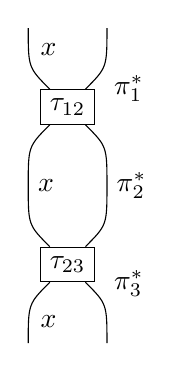
\begin{tikzpicture}[baseline=(current bounding box.center),]
\path coordinate[] (tikzsd_internal_pos_0_0) at (0.0,0.0);
\path coordinate[] (tikzsd_internal_pos_0_1) at (1.0,0.0);
\path coordinate[] (tikzsd_internal_pos_1_0) at (0.0,-2.0);
\path coordinate[] (tikzsd_internal_pos_1_1) at (1.0,-2.0);
\path coordinate[] (tikzsd_internal_pos_2_0) at (0.0,-4.0);
\path coordinate[] (tikzsd_internal_pos_2_1) at (1.0,-4.0);

\path node[,draw,] (tikzsd_internal_nt_node_0_0) at (0.5,-1.0) {$\tau_{12}$};
\path node[,draw,] (tikzsd_internal_nt_node_1_0) at (0.5,-3.0) {$\tau_{23}$};

\path [draw] (tikzsd_internal_pos_0_0) ..controls(0.0,-0.5)..(tikzsd_internal_nt_node_0_0) node[pos=0.5,auto,] {$x$};
\path [draw] (tikzsd_internal_pos_0_1) ..controls(1.0,-0.5)..(tikzsd_internal_nt_node_0_0) node[pos=0.5,auto,] {$\pi_1^\ast$};
\path [draw] (tikzsd_internal_nt_node_0_0) ..controls(0.0,-1.5)..(tikzsd_internal_pos_1_0) ..controls(0.0,-2.5)..(tikzsd_internal_nt_node_1_0) node[pos=0.0,auto,] {$x$};
\path [draw] (tikzsd_internal_nt_node_0_0) ..controls(1.0,-1.5)..(tikzsd_internal_pos_1_1) ..controls(1.0,-2.5)..(tikzsd_internal_nt_node_1_0) node[pos=0.0,auto,] {$\pi_2^\ast$};
\path [draw] (tikzsd_internal_nt_node_1_0) ..controls(0.0,-3.5)..(tikzsd_internal_pos_2_0) node[pos=0.5,auto,] {$x$};
\path [draw] (tikzsd_internal_nt_node_1_0) ..controls(1.0,-3.5)..(tikzsd_internal_pos_2_1) node[pos=0.5,auto,] {$\pi_3^\ast$};
\end{tikzpicture}